%!TEX encoding = UTF-8
\documentclass[uplatex]{jsarticle}
\usepackage{siunitx}
\usepackage{datetime}
% \usepackage[T1]{fontenc}
\usepackage{titlesec}
\usepackage{multirow}
\usepackage{amsmath, amssymb}
\usepackage{docmute}
\usepackage[dvipdfmx]{graphicx}
\usepackage{hhline}
\usepackage{mathtools}
\usepackage{amsmath}
\usepackage{here}
\usepackage{graphicx}
\usepackage{listings, jlisting}
\usepackage{subfig}

% ページをまたぐ長い表を作成する by http://wright.mydns.jp/?p=1015
\usepackage{longtable}

\renewcommand{\lstlistingname}{プログラムリスト}

\usepackage{latexsym}
\usepackage{bmpsize}
\usepackage{url}
\usepackage{comment}
% \usepackage{pdfpages}

\lstset{
  basicstyle={\ttfamily},
  identifierstyle={\small},
  commentstyle={\small\itshape},
  keywordstyle={\small\bfseries},
  ndkeywordstyle={\small},
  stringstyle={\small\ttfamily},
  frame={tb},
  breaklines=true,
  columns=[l]{fullflexible},
  numbers=left,
  xrightmargin=0zw,
  xleftmargin=3zw,
  numberstyle={\scriptsize},
  stepnumber=1,
  numbersep=2zw,
  lineskip=-0.5ex,
  tabsize=4
}

\begin{document}
  \newpage
  % !TEX root = ../main.tex
\begin{document}

\section{実験の目的}
  情報技術基礎、およびプログラミングIの授業で習得したC言語を用いて、与えられた仕様を満たすプログラムを各自が自由に設計を行い作成する。
  プログラムの作成にあたり、処理手順の検討、フローチャートの記述、プログラムの作成、デバッグ、テストを完了させるというソフトウェア開発の一連の流れを実践する。

\end{document}

  % !TEX root = ../main.tex
\begin{document}

\section{実験の概要}
\subsection{平方採中法について}
  平方採中法とは、1940年代にノイマンによって提案された、擬似乱数を生成するための古典的手法である。
  例えば、求めたい乱数の桁数を最大で4桁とし、乱数の初期値を6184とすると、次のような手順で順次求められる。

  \begin{align*}
    6174^2 = 38118276 → 1182 \\
    1182^2 = 01397124 → 3971 \\
    3971^2 = 15768841 → 7688
  \end{align*}

  このような、与えられた値を二乗し、その間の特定の桁を乱数として採用し、
  その値を次の初期値として擬似乱数を算出するのが、平方採中法である。

\subsection{作成するプログラムの仕様}
  \subsubsection{入力}
    入力された$n$を初期値として、平方採中法により求められた10個の擬似乱数、
    ここでは、最大で4桁の擬似乱数を求めるものとする。


\end{document}

  % !TEX root = ../main.tex
\begin{document}
\section{作成したフローチャート}
作成したフローチャートを図\ref{作成したフローチャート}に示す。

\begin{figure}[H]
    \centering
    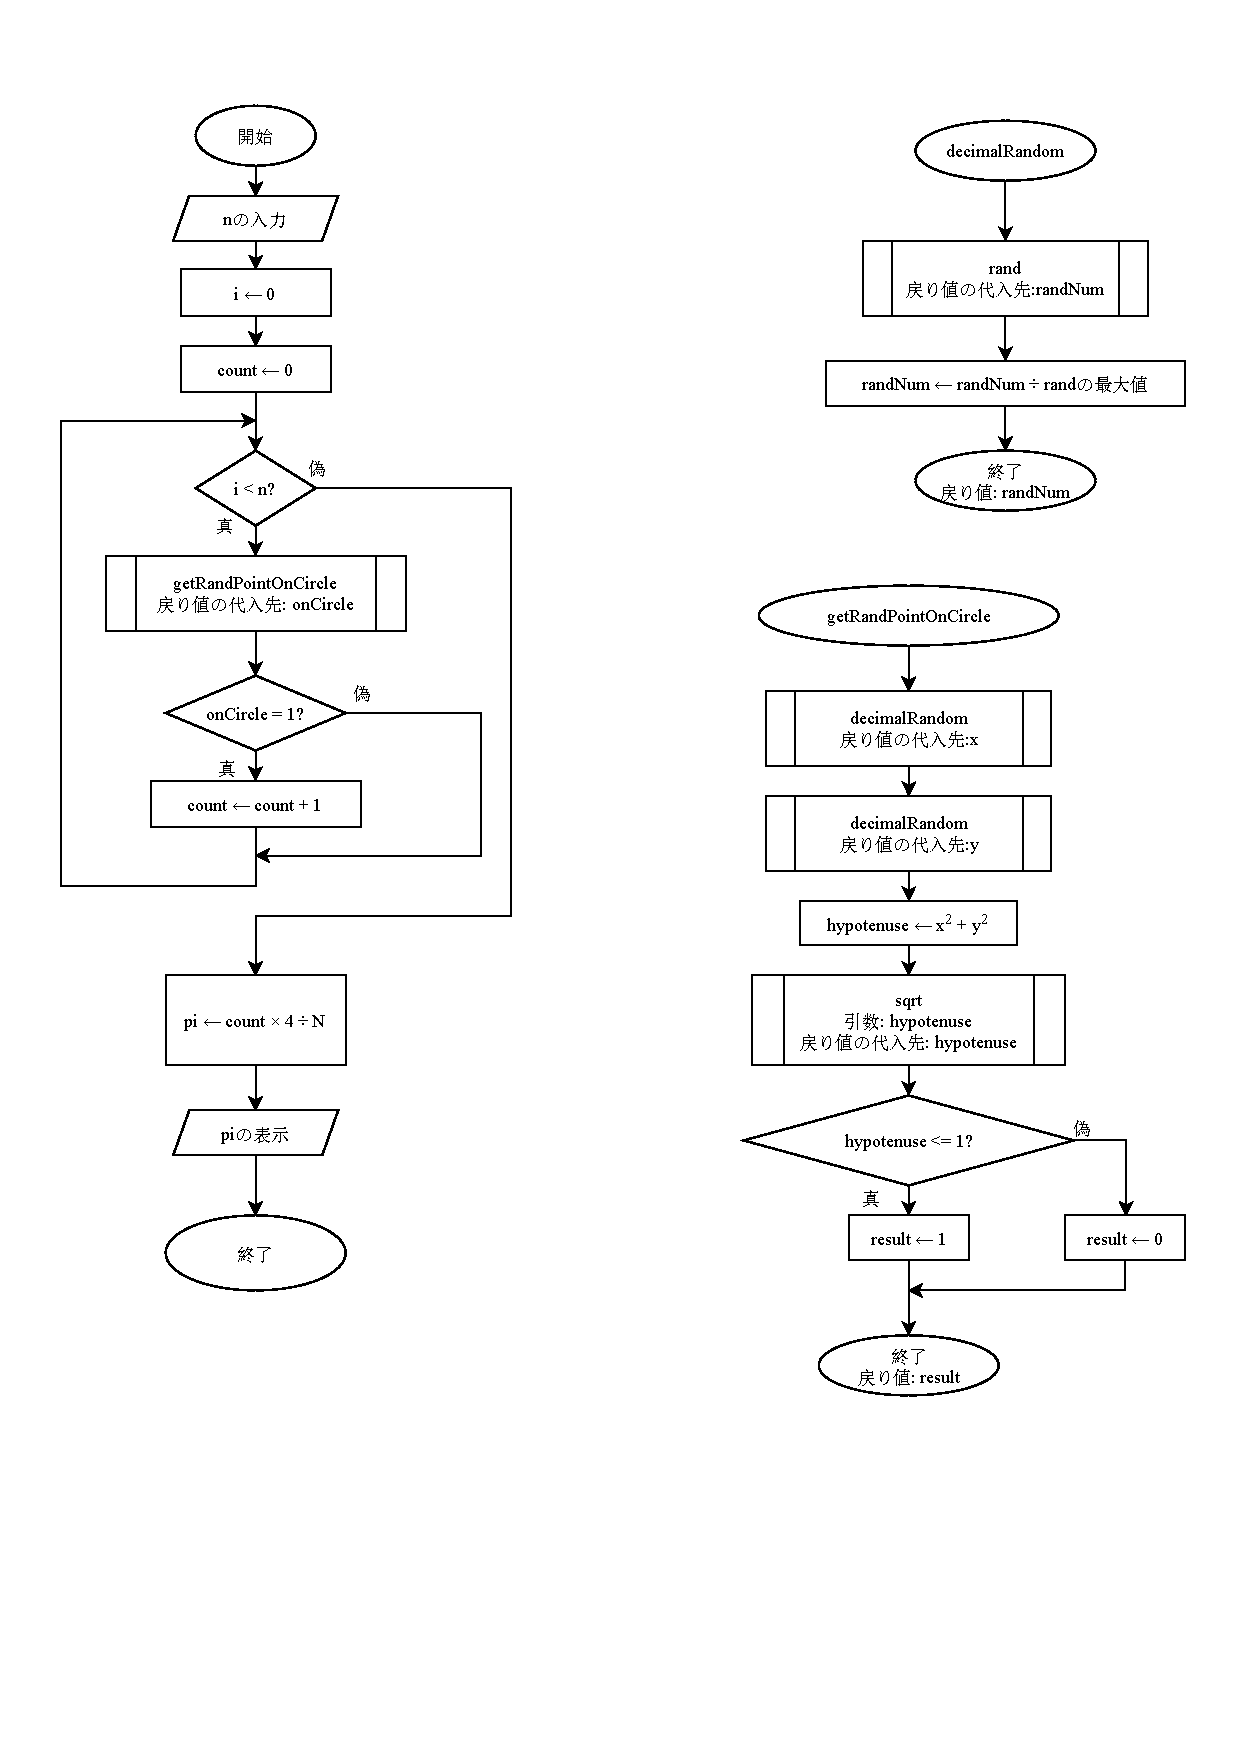
\includegraphics[width=0.8\hsize,pagebox=mediabox, page=1]{flowchart.pdf}
    \label{作成したフローチャート}
    \caption{作成したフローチャート}
\end{figure}

\end{document}

  % !TEX root = ../main.tex
\begin{document}

\section{作成したプログラムの全リスト}
作成したプログラムをプログラム1に示す。

\lstinputlisting[caption=作成したプログラム,language=C]{./main.c}

\end{document}

  % !TEX root = ../main.tex
\begin{document}

\section{作成したプログラムの説明}
まず、``初期値: ''を標準出力へ表示した上で、
標準入力からの読み込みを行う。

指示より、10個の擬似乱数を作成、表示するため、10回の繰り返し処理を行い、終了する。

繰り返し処理の内容を以下に示す。

まず、乱数の元となる数を二乗する。
その数から、以下の式を用いて、2桁目から6桁目までの数を算出した。
元にする数を$n^2$とする
\begin{align*}
    (n^2 \div 100) \bmod 10000
\end{align*}

算出した値を、元となる数へ代入した上で、
値を標準入力に表示した。

\end{document}

  % !TEX root = ../main.tex
\begin{document}

\section{ソフトウェアテストの結果について}
入力内容と期待される出力内容を表\ref{入力内容と期待される出力内容}に示す。

\begin{table}[H]
    \centering
    \caption{入力内容と期待される出力内容}
    \label{入力内容と期待される出力内容}
        \begin{tabular}{|c|c|} \hline
            入力内容 & 期待される出力内容 \\ \hline
            0001 & 5 \\
            2447 & 6 \\
            3883 & 5 \\
            7676 & 4 \\
            9592 & 4 \\
            9999 & 1 \\ \hline
        \end{tabular}
\end{table}

以下より、作成したプログラムが正しく動作することを確認した。

\$ ./s-1.out \\
正の整数(4桁)の入力: 9999 \\
1 \\
\\
\$ ./s-1.out \\ 
正の整数(4桁)の入力: 9552 \\ 
4 \\
\\
\$ ./s-1.out \\
正の整数(4桁)の入力: 2447 \\
6 \\
\\
\$ ./s-1.out \\
正の整数(4桁)の入力: 7676 \\
4 \\
\\
\$ ./s-1.out \\
正の整数(4桁)の入力: 3883 \\
5 \\
\\
\$ ./s-1.out \\
正の整数(4桁)の入力: 9999 \\
1 \\

\end{document}


  % !TEX root = ../main.tex
\begin{document}

\section{発生したエラーや不具合およびそれらの原因と対策方法}
最初のコンパイル時、関数が存在しないというエラーが発生した。
このエラーの原因は使用する関数を、その前に定義するか、プロトタイプ宣言を行わなければ行けないというのを忘れていたことである。
main関数定義の上でプロトタイプ宣言を行うことで対策を行った。



\end{document}

  % !TEX root = ../main.tex
\begin{document}

\section{実験で工夫したこと・実験から学んだこと}
最初には30行目でsqrt関数を用いて以下の式を参考に実装していた。
\begin{align*}
  \sqrt{x^2 + y^2} \leqq 1
\end{align*}

この式は両辺を自乗して以下のように変更可能である。
\begin{align*}
  x^2 + y^2 \leqq 1
\end{align*}
この式を用いると平方根の計算を行わなくて良いため、計算にかかる時間を削減できる工夫を行った。

\end{document}

  % !TEX root = ../main.tex
\begin{document}

\section{感想}
  コンピュータによる円周率の計算方法の一つを知ることができ、興味深く感じた。
  また、計算量の削減による実行時間の短縮も考慮したプログラムを作成していきたい。

\end{document}
  % % !TEX root = ../main.tex
\begin{document}

\section{参考文献}
【C言語/C++】 配列は戻り値にできない【配列を適切に返す方法】 \\
https://marycore.jp/prog/c-lang/return-array/ \\
最終閲覧日 2019/12/04

昇順と降順 \\
https://www.pc-master.jp/words/shojyun-kojyun.html \\
最終閲覧日 2019/12/04

配列をコピーする Programming Place Plus C言語編 逆引き \\
https://programming-place.net/ppp/contents/c/rev\_res/array004.html \\
最終閲覧日 2019/12/04

The pow functions - pow, powf, powl \\
http://www.c-tipsref.com/reference/math/pow.html \\
最終閲覧日 2019/12/04

ある数のn桁目の値を取り出す関数 \\
https://detail.chiebukuro.yahoo.co.jp/qa/question\_detail/q1090279785 \\
最終閲覧日 2019/12/04

関数に配列を渡す \\
http://www.ie.u-ryukyu.ac.jp/~e075769/study/study/c/ch7/7\_10.php \\
最終閲覧日 2019/12/04

\end{document}

\end{document}
